\documentclass[a4paper,10pt]{ctexart}
%引用设置使用Bibtex
\usepackage{gbt7714}
\bibliographystyle{gbt7714-numerical}
%页面设置
\usepackage{geometry}
%字体设置
\usepackage{fontspec}
%\setmainfont{Times New Roman}
%定理环境
\usepackage{amsmath}
%\numberwithin{equation}{section}
\usepackage{amsthm}
\newtheorem*{definition}{Definition}
\newtheorem*{theorem}{Theorem}
\newtheorem*{corollary}{Corollary}
\newtheorem*{proposition}{Proposition}
\newtheorem*{example}{Example}
%数学环境字体
\usepackage{bm}
\usepackage[all]{xy}
%加载 TikZ 用于绘制交换图
\usepackage{tikz-cd}
%颜色
\usepackage{color,xcolor}

\definecolor{miku}{RGB}{57,197,187}
\definecolor{sakura}{RGB}{255,192,203}
\definecolor{rose}{RGB}{255,228,225}
\definecolor{brown}{RGB}{210,105,30}
\definecolor{lbrown}{RGB}{239,235,224}
\definecolor{bule}{RGB}{0,47,167}
\definecolor{lyellow}{RGB}{250,250,210}
\definecolor{lpurple}{RGB}{255,240,245}
\definecolor{lbule}{RGB}{135,206,250}
\definecolor{gbule}{RGB}{64,224,208}
\definecolor{green}{RGB}{138,200,207}
\definecolor{lgreen}{RGB}{225,255,255}
\definecolor{lorange}{RGB}{248,172,140}
\definecolor{salmon}{RGB}{250,128,114}
\definecolor{burgundy}{rgb}{0.5, 0.0, 0.13}
%链接设置
\usepackage[colorlinks=true,pdfstartview=FitH,linkcolor=blue,anchorcolor=violet, citecolor=magenta]{hyperref} 
%封面
\usepackage{pdfpages}
\usepackage{mathrsfs}
\usepackage{amssymb}
\usepackage{graphicx}
\usepackage{lipsum}
%彩色框
\usepackage{framed}
\usepackage{tcolorbox}
\tcbuselibrary{breakable}
\tcbuselibrary{theorems}
\tcbuselibrary{skins}
\usepackage{colortbl}
\usepackage{float}
\usepackage[export]{adjustbox}
\newtcolorbox[auto counter,number within=section]{notebox}[2][]{%
colback=miku!2!white,
colframe=miku,
coltitle=white,
fonttitle=\bfseries,
rightrule=2pt,
leftrule=2pt,
bottomrule=2pt,
colbacktitle=miku,
theorem style=standard,
breakable,
arc=2pt,
drop fuzzy shadow=black!20!white,
title=Note~\thetcbcounter: #2,#1}
\newtcolorbox[auto counter,number within=section]{markbox}[2][]{%
colback=miku!2!white,
colframe=miku,
coltitle=white,
fonttitle=\bfseries,
rightrule=0pt,
leftrule=0pt,
bottomrule=2pt,
colbacktitle=miku,
theorem style=standard,
breakable,
arc=0pt,
drop fuzzy shadow=black!20!white,
title=Remark~\thetcbcounter: #2,#1}
\newtcolorbox[no counter]{theorems}[2][]{%
width=12cm,
center,
sidebyside,
sidebyside adapt=left,
sidebyside gap=6mm,
sidebyside align=center seam,
colback=burgundy!2!white,
colframe=burgundy,
coltitle=white,
fonttitle=\bfseries,
rightrule=1pt,
leftrule=1pt,
bottomrule=2pt,
colbacktitle=burgundy,
theorem style=standard,
enhanced,
drop fuzzy shadow southeast=black!30!white,
breakable,
arc=0pt,
title=Theorem. #2,#1}
\newtcolorbox[no counter]{definitions}[2][]{%
width=12cm,
center,
colback=lyellow!2!white,
colframe=yellow!3!lyellow,
coltitle=bule,
fonttitle=\bfseries,
rightrule=0pt,
leftrule=1pt,
bottomrule=2pt,
colbacktitle=lyellow,
theorem style=standard,
breakable,
arc=5pt,
enhanced,
drop fuzzy shadow southeast=black!20!white,
title=Definition. #2,#1}
\newtcolorbox[auto counter,number within=section]{corollarys}[2][]{%
colback=lyellow!2!white,
colframe=lyellow,
coltitle=bule,
fonttitle=\bfseries,
rightrule=0pt,
leftrule=1pt,
bottomrule=2pt,
colbacktitle=lyellow,
theorem style=standard,
breakable,
arc=0pt,
enhanced,
drop fuzzy shadow southeast=black!20!white,
title=Corollary~\thetcbcounter: #2,#1}
\newtcolorbox[auto counter,number within=section]{lemmas}[2][]{%
width=12cm,
center,
colback=lyellow!2!white,
colframe=lorange!30!sakura,
coltitle=bule,
fonttitle=\bfseries,
rightrule=0pt,
leftrule=1pt,
bottomrule=2pt,
colbacktitle=lorange!30!sakura,
theorem style=standard,
breakable,
arc=5pt,
enhanced,
drop fuzzy shadow southeast=black!20!white,
title=Lemma. #2,#1}
\newtcolorbox[auto counter,number within=section]{propositions}[2][]{%
width=12cm,
center,
colback=salmon!5,
colframe=salmon!90!black,
coltitle=white,
fonttitle=\bfseries,
rightrule=1pt,
leftrule=1pt,
bottomrule=2pt,
colbacktitle=salmon!90!black,
theorem style=standard,
breakable,
arc=5pt,
enhanced,
drop fuzzy shadow southeast=black!20!white,
title=Proposition. #2,#1}
\newtcolorbox[no counter]{egbox}[2][]{%
width=12cm,
center,
colback=black!5!white,
colframe=black!20!white,
coltitle=black,
fonttitle=\bfseries,
rightrule=1pt,
leftrule=1pt,
bottomrule=2pt,
colbacktitle=black!20!white,
theorem style=standard,
breakable,
arc=0pt,
enhanced,
drop fuzzy shadow southeast=black!20!white,
title=Example. #2,#1}

%\begin{figure}[H]
%\centering
%\includegraphics[center]{pic.png}
%\end{figure}
\geometry{left=3cm,right=3cm,top=2cm,bottom=2cm}
\tcbuselibrary{most}

%自定义设置
\renewcommand{\proofname}{Proof.}
\renewcommand{\contentsname}{ Content }
\newcommand{\image}[2]{
    \centering
    \includegraphics[width={#1}\textwidth]{#2}
}



\newcommand\keywords[1]{\vskip2ex\par\noindent\normalfont{\textbf{关键词}: #1}}
\newcommand{\ekeywords}[1]{\vskip2ex\par\noindent\normalfont{\bfseries Key Words: }#1}
\newcommand{\miku}{\textcolor{miku}}
\newcommand{\sakura}{\textcolor{sakura}}
\newcommand{\brown}{\textcolor{brow}}
\newcommand{\red}{\textcolor{red}}
\newcommand{\blue}{\textcolor{blue}}
\newcommand{\A}{\mathcal{A}}
\newcommand{\C}{\mathbb{C}}
\newcommand{\al}{\alpha}
\newcommand{\sa}{$\sigma$-algebra}
\newcommand{\Bsa}{Borel $\sigma$-algebra}
\newcommand{\F}{\mathcal{F}}
\newcommand{\N}{\mathcal{N}}
\newcommand{\M}{\mathcal{M}}
\newcommand{\m}{ $\mathcal{M}$ }
\newcommand{\B}{\mathcal{B}}
\newcommand{\myP}{\mathcal{P}}
\renewcommand{\bf}[1]{\textbf{#1}}

\newcommand{\myRom}[1]{\uppercase\expandafter{\romannumeral#1}}
\newcommand{\pl}{$ L^p(X) $}
\newcommand{\twol}{$ L^2(X) $}
\usepackage{booktabs}
\pgfplotsset{compat=1.18}

\begin{document}
\hfill\vbox{\hbox{Numerical Analysis}\hbox{陈曦,HOME}\hbox{Summer, 2024}}

\begin{center}\Large
    \textbf{数值分析}\\{\normalsize\bf {多项式插值和逼近}}
\end{center}
\vskip 30pt
\small {参考书目:
\begin{itemize}
    \item Numerical Analysis(David Kincaid, Ward Cheney)
    \item Numerical Analysis(Timothy Sauer,2014)
    \item Approximation Theory and Approximation Practice(Trefethen,2013)
\end{itemize}}
\vskip 30pt

\section{多项式插值}
多项式插值是最基础也应用最广泛的数值方法之一。给定一些数据点,多项式插值的目标是找到一个多项式,使得这个多项式通过所有的数据点,以下插值基本定理保证了这样的多项式的存在性和唯一性。
\begin{theorem}
    给定$n+1$个不同的数据点$(x_0,y_0),\ldots,(x_n,y_n)$,其中$x_0,\ldots,x_n$是互不相同的实数,那么存在唯一的次数不超过$n$的多项式$p(x)$,使得$p(x_i)=y_i$,$i=0,\ldots,n$。
\end{theorem}
\noindent 稍后我们将构造性地给出这种相应的多项式以证明存在性,唯一性的证明只需注意到具有$ n+1 $个零点的$ n $阶多项式只能是零多项式。

常用的插值方法包括Newton插值、Lagrange插值和Hermite插值。Newton插值是递推方法,比较方便插入新的插值节点,Lagrange插值可以显式地直接构造,并且可以写成质心公式的形式,最后与前两者不同,Hermite插值不仅使用了极点函数值,还可以进一步利用插值节点处的导数信息。

\subsection{Lagrange插值}
Lagrange插值是最直接的插值方法,给定插值点$ x_0,\cdots x_n $以及这些点上的函数值$ f(x_0),\cdots ,f(x_n) $,我们定义Lagrange插值基函数
\begin{equation}
    \ell_i(x)=\prod_{j=0,j\neq i}^{n}\frac{x-x_j}{x_i-x_j},
\end{equation}
于是Lagrange插值多项式为
\begin{equation}
    L(x)=\sum_{i=0}^{n}f(x_i)\ell_i(x).
\end{equation}

现在我们对Lagrange插值多项式的插值误差进行估计。首先注意到
\[
    f(x_i) = L(x_i),\quad i=0,\cdots,n,
\]
因此$ x_0,\cdots ,x_n $是$ L(x)-f(x) $的$ n+1 $个零点,由此可知存在$ K $使得
\begin{equation}
    L(x)-f(x)=K(x)\prod_{i=0}^{n}(x-x_i),
\end{equation}
下面我们考虑分析$ K(x) $。令$ a $为$ f $的定义域中的任意一点,现在构造辅助函数:
\begin{equation}
    \phi(x)=f(x)-L(x)-K(a)\prod_{i=0}^{n}(x-x_i),
\end{equation}
显然$ \phi(x) $在$ x_0,\cdots,x_n $和$ a $处都为零,当$ \phi $在足够大的区间上连续且存在导函数时,根据Rolle定理可知在相邻的零点之间存在$ \xi_k $使得$ \phi'(\xi_k)=0 $,这样我们得到了$ \phi' $的$ n+1 $个零点,进一步要求$ \phi' $也在足够大的区间上连续且可导,则再次应用Rolle定理可得$ \phi'' $的$ n $个零点,以此类推,最终我们得到了$ \phi^{(n+1)} $的一个零点,记为$ \xi $。注意到$ L $是$ n $次多项式,因此$ L^{(n+1)}=0 $,所以
\begin{equation}
    \phi^{(n+1)}(\xi)=f^{(n+1)}(\xi)-K(a)(n+1)!=0,
\end{equation}
由此可知
\begin{equation}
    K(a) = \frac{f^{(n+1)}(\xi)}{(n+1)!}
\end{equation}
对任意$ a $成立,因此$ K(x) $是一个常数,即
\begin{equation}
    K = \frac{f^{(n+1)}(\xi)}{(n+1)!},
\end{equation}
这样我们就得到了Lagrange插值多项式的插值误差:
\begin{equation}
    L(x)-f(x)=\frac{f^{(n+1)}(\xi)}{(n+1)!}\prod_{i=0}^{n}(x-x_i).
\end{equation}
注意上述证明依赖于被插值函数$ f(x) $的光滑性。

\begin{theorem}
    当被插值函数$ f(x) $的$ n+1 $阶导数存在且连续时,$ n $阶Lagrange插值多项式$ L_n(x) $满足如下误差估计
    \begin{equation}
        f(x)-L_n(x)=\frac{f^{(n+1)}(\xi)}{(n+1)!}\prod_{i=0}^{n}(x-x_i).
    \end{equation}
\end{theorem}

更多分析参见\href{http://staff.ustc.edu.cn/~rui/ppt/num/num-interpolation-lagrange.html}{Lagrange插值}。

\subsection{Newton插值}
给定插值点$ x_0,\cdots x_n $以及这些点上的函数值$ f(x_0),\cdots ,f(x_n) $,首先我们递推地定义差商,令
\begin{equation}
    f[x_i]=f(x_i),\quad f[x_i,x_{i+1}]=\frac{f[x_{i+1}]-f[x_i]}{x_{i+1}-x_i},
\end{equation}
并且
\begin{equation}
    f[x_i,\cdots,x_{i+k}]=\frac{f[x_{i+1},\cdots,x_{i+k}]-f[x_i,\cdots,x_{i+k-1}]}{x_{i+k}-x_i},
\end{equation}
使用数学归纳法将差商展开可得
\begin{equation}
    f[x_0,\cdots,x_k]=\sum_{i=0}^k \frac{f(x_i)}{(x_i-x_0)\cdots (x_i-x_{i-1})(x_i-x_{i+1})\cdots (x_i-x_k)}
\end{equation}
由此可见按照如上方法定义的差商与使用插值点的顺序无关,即
\[
    f[x_0,x_1,\cdots,x_k]=f[x_{i_0},x_{i_1},\cdots,x_{i_k}],
\]
其中$ i_0,\cdots,i_k $是$ 0,\cdots,k $的任意重排。

通常计算差商按照如下的差商表进行:
\begin{center}
    \begin{tabular}{ccccc}
        \toprule
        $x_i$ & $f[x_i]$ & $f[x_i,x_{i+1}]$ & $f[x_i,x_{i+1},x_{i+2}]$ & $f[x_i,x_{i+1},x_{i+2},x_{i+3}]$ \\
        \midrule
        $x_0$ & $f(x_0)$ &  &  & \\
        $x_1$ & $f(x_1)$ & $f[x_0,x_1]$ & & \\
        $x_2$ & $f(x_2)$ & $f[x_1,x_2]$ & $f[x_0,x_1,x_2]$ & \\
        $x_3$ & $f(x_3)$ & $f[x_2,x_3]$ & $f[x_1,x_2,x_3]$ & $f[x_0,x_1,x_2,x_3]$ \\
        \bottomrule
    \end{tabular}
\end{center}

借助这些差商,我们可以定义Newton插值多项式
\begin{equation}
    N(x)=\sum_{k=0}^{n}f[x_0,\cdots,x_{k}]\prod_{i=0}^{k-1}(x-x_i).
\end{equation}

关于Newton插值多项式,我们有如下Newton插值定理:
\begin{theorem}
    当被插值函数$ f(x) $满足一定的光滑性要求时,$ n $阶Newton插值多项式$ N(x) $满足插值误差估计
    \begin{equation}
        f(x)-N_n(x)=f[x_0,\cdots,x_n,\textcolor{red}{x}] \prod_{i=0}^{n}(x-x_i).
    \end{equation}
\end{theorem}
\begin{proof}
    使用数学归纳法进行证明。当$ n=0 $时我们有
    \[
        f[x_0,x] = \frac{f(x)-f(x_0)}{x_1-x_0} ,
    \]
    此即
    \[
        f(x) = f(x_0) + f[x_0,x](x-x_0),
    \]
    因此命题成立。假设命题对$ n-1 $阶插值多项式成立,即
    \[
        f(x)-N_{n-1}(x)=f[x_0,\cdots,x_{n-1},x] \prod_{i=0}^{n-1}(x-x_i),
    \]
    现在我们考虑$ n $阶插值多项式$ p_n(x) $,有
    \[
        N_n(x)=N_{n-1}(x)+f[x_0,\cdots,x_n]\prod_{i=0}^{n-1}(x-x_i),
    \]
    由此可得
    \[
        f(x)-N_n(x)=f[x_0,\cdots,x_{n-1},x]\prod_{i=0}^{n-1}(x-x_i) - f[x_0,\cdots,x_n]\prod_{i=0}^{n-1}(x-x_i).
    \]
    注意到
    \[
        f[x_0,\cdots,x_n,x] = f[x_n,x_0,\cdots,x_{n-1},x] = \frac{f[x_0,\cdots ,x_n]-f[x_0,\cdots ,x_{n-1},x]}{x_n-x},
    \]
    此即
    \[
        f[x_0,\cdots,x_{n-1},x] = f[x_0,\cdots,x_n] + f[x_0,\cdots,x_n,x](x-x_n),
    \]
    带入$ f(x)-p_n(x) $可知
    \[
        f(x)-N_n(x)=f[x_0,\cdots,x_n,x]\prod_{i=0}^{n}(x-x_i),
    \]
    因此阶数为$ n $时命题成立,由数学归纳法可知命题对所有$ n $成立。
\end{proof}

当需要添加新的插值节点时,可以将新加入的节点和函数值对记为$ (x_{-1},f(x_{-1})) $,于是新的差商表为
\begin{center}
    \begin{tabular}{cccccc}
        \toprule
        $x_i$ & $f[x_i]$ & $f[x_i,x_{i+1}]$ & $f[x_i,x_{i+1},x_{i+2}]$ & $f[x_i,x_{i+1},x_{i+2},x_{i+3}]$ & $f[x_i,x_{i+1},x_{i+2},x_{i+3},x_{i+4}]$ \\
        \midrule
        $\textcolor{blue}{x_{-1}}$ & $\textcolor{blue}{f(x_{-1})}$ & & & & \\
        $x_0$ & $f(x_0)$ & $\textcolor{blue}{f[x_{-1},x_0]}$ & & & \\
        $x_1$ & $f(x_1)$ & $f[x_0,x_1]$ & $\textcolor{blue}{f[x_{-1},x_0,x_1]}$ & & \\
        $x_2$ & $f(x_2)$ & $f[x_1,x_2]$ & $f[x_0,x_1,x_2]$ & $\textcolor{blue}{f[x_{-1},x_0,x_1,x_2]}$ & \\
        $x_3$ & $f(x_3)$ & $f[x_2,x_3]$ & $f[x_1,x_2,x_3]$ & $f[x_0,x_1,x_2,x_3]$ & $\textcolor{blue}{f[x_{-1},x_0,x_1,x_2,x_3]}$ \\
        \bottomrule
    \end{tabular}
\end{center}
所以为了得到新的插值多项式只需计算最外层的差商即可,而这些差商的计算只依赖于次外层的差商(在实际计算中我们只需储存最外侧差商,覆盖到函数值向量$ y $上以节省内存占用),因此Newton插值对于添加新的插值节点是非常高效的。

更多分析参见\href{http://staff.ustc.edu.cn/~rui/ppt/num/num-interpolation-newton.html}{Newton插值}。

\subsection{Hermite插值}
如果问题除了给定插值节点$ x_0,\cdots ,x_n $和对应的函数值$ f(x_0),\cdots ,f(x_n) $外,还给定了各插值格点上的导数信息:在$ x_i $上已知$ f^{(j)}(x_i) $,其中$ j=1,\cdots ,p_i $,则相应的Hermite插值多项式$ H $需要满足
\begin{equation}
    H^{(j)}(x_i) = f^{(j)}(x_i),\quad j=0,\cdots ,p_i,\quad i=0,\cdots ,n.
\end{equation}

比较常用的计算Hermite插值多项式的方法是基函数法,与Lagrange插值和Newton插值类似,当给定$ (p_1+1)+\cdots +(p_n+1) $个插值条件之后,所可以确定的Hermite插值多项式的阶数至多为$ (p_1+1)+\cdots +(p_n+1)-1 $,现在希望找到一组基函数$ h_{ij}(x) $,使得Hermite插值多项式可以表示为
\begin{equation}
    H(x)= \sum_{i=0}^{n} \sum_{j=0}^{p_i}f^{(j)}(x_i) h_{ij}(x).
\end{equation}
我们以二重切触插值和三重切触插值为例说明如何使用基函数法计算Hermite插值多项式。

\begin{example}
    考虑二重切触插值问题:给定插值节点$ x_0,\cdots ,x_n $,以及在$ x_i $上的函数值$ f(x_i) $和导数值$ f'(x_i) $,我们希望找到一个次数不超过$ 2n+1 $的多项式$ H(x) $,使得
    \[
        H(x_i)=f(x_i),\quad H'(x_i)=f'(x_i),\quad i=0,\cdots ,n.
    \]
    上述条件包含$ 2n+2 $个插值要求,因此Hermite多项式至多$ 2n+1 $阶,于是设Hermite多项式形如
    \begin{equation}
        H(x)=\sum_{i=0}^{n}f(x_i)\alpha_i(x)+\sum_{i=0}^{n}f'(x_i)\beta_i(x),
    \end{equation}
    其中$ \alpha_i(x) $和$ \beta_i(x) $是$ 2n+1 $阶的基函数,满足
    \[
        \alpha_i(x_j)=\delta_{ij},\quad \alpha_i'(x_j)=0,\quad \beta_i(x_j)=0,\quad \beta_i'(x_j)=\delta_{ij}.
    \]
    基函数的构造不唯一,注意到对于$ \alpha_i $而言所有节点处的导数为零且只有$ x_i $处函数值非零为$ 1 $,因此希望寻找形如
    \begin{equation}
        \alpha_i(x) = (a_ix+b_i)l^2_i(x)
    \end{equation}
    的基函数,其中$ l_i $是第$ i $个Lagrange基函数,带入插值条件还需要求
    \[
        (a_ix_i+b_i)l^2_i(x_i) = 1,\quad l_i(x_i)[a_il_i(x_i)+2(a_ix_i+b_i)l_i'(x_i)] = 0,
    \]
    注意到$ l_i(x_i)=1 $,于是
    \[
        a_ix_i+b_i = 1,\quad a_i +2 l_i'(x_i) = 0,
    \]
    由此可得基函数系数为
    \begin{equation}
        a_i = -2l_i'(x_i),\quad b_i = 1+2x_il_i'(x_i).
    \end{equation}
    回忆
    \[
        l_i'(x) = \frac{d}{dx} \prod_{j=0,j\neq i}^{n}\frac{x-x_j}{x_i-x_j},
    \]
    于是
    \[
        l_i'(x_i) = \sum_{j=0,j\neq i}^{n}\frac{1}{x_i-x_j},
    \]
    因此
    \begin{equation}
        \begin{aligned}
            \alpha_i(x) 
            &= \left( -2x\sum_{j=0,j\neq i}^{n}\frac{1}{x_i-x_j} + 1+2x_i\sum_{j=0,j\neq i}^{n}\frac{1}{x_i-x_j} \right) l_i^2(x)\\
            &= \left( 1-2(x-x_i)\sum_{j=0,j\neq i}^{n}\frac{1}{x_i-x_j} \right) l_i^2(x)
        \end{aligned}
    \end{equation}
    类似地,对于$ \beta_i $我们希望寻找形如
    \begin{equation}
        \beta_i(x) = (c_ix+d_i)l^2_i(x)
    \end{equation}
    的基函数,带入插值条件还需要求
    \[
        (c_ix_i+d_i)l^2_i(x_i) = 0,\quad l_i(x_i)[c_il_i(x_i)+2(c_ix_i+d_i)l_i'(x_i)] = 1,  
    \]
    可解出
    \[
        c_i = 1,\quad d_i = -x_i,
    \]
    所以
    \begin{equation}
        \beta_i(x) = (x-x_i)l^2_i(x).
    \end{equation}
    至此我们得到了二重切触插值的基函数,进而可以构造Hermite插值多项式。
\end{example}

与二重切触插值类似,三重切触插值的基函数可以通过类似的方法构造,不过此时基函数的阶数会更高,因此计算会更加复杂。我们这里只考虑两点情况。

\begin{example}
    考虑两点三重切触插值问题:给定插值节点$ x_0,x_1 $,以及在$ x_i $上的函数值$ f(x_i) $和导数值$ f'(x_i) $和二阶导数值$ f''(x_i) $,我们希望找到一个次数不超过$ 3n+2 = 5 $的多项式$ H(x) $,使得
    \[
        H(x_i)=f(x_i),\quad H'(x_i)=f'(x_i),\quad H''(x_i)=f''(x_i),\quad i=0,\cdots ,n.
    \]
    上述条件包含$ 3n+3 = 6 $个插值要求,因此Hermite多项式至多$ 3n+2 = 5 $阶,于是设Hermite多项式形如
    \begin{equation}
        H(x)=\sum_{i=0}^{1}f(x_i)\alpha_i(x)+\sum_{i=0}^{1}f'(x_i)\beta_i(x)+\sum_{i=0}^{1}f''(x_i)\gamma_i(x),
    \end{equation}
    其中$ \alpha_i(x) $、$ \beta_i(x) $和$ \gamma_i(x) $是$ 3n+2=5 $阶的基函数,满足
    \[
        \begin{aligned}
            \alpha_i(x_j)=\delta_{ij},\quad \alpha_i'(x_j)=0,\quad \alpha_i''(x_j)=0,\\
            \beta_i(x_j)=0,\quad \beta_i'(x_j)=\delta_{ij},\quad \beta_i''(x_j)=0,\\
            \gamma_i(x_j)=0,\quad \gamma_i'(x_j)=0,\quad \gamma_i''(x_j)=\delta_{ij}.
        \end{aligned}
    \]
    基函数的构造不唯一,注意到对于$ \alpha_i $而言所有节点处的导数为零且只有$ x_i $处函数值非零为$ 1 $,因此可以选取
    \begin{equation}
        \alpha_i(x) = (a_ix^2+b_ix+c_i)l^3_i(x),
    \end{equation}
    还需满足
    \[
        \begin{aligned}
            a_ix_i^2+b_ix_i+c_i = 1,\\
            (2a_ix_i+b_i)+3l_i'(x_i) = 0,\\
            2a_il_i^3(x_i)+6(2a_ix_i+b_i)l_i^2(x_i) l_i'(x_i) + 3(2(l_i'(x_i))^2+l_i^2(x_i)l_i'(x_i)) = 0,
        \end{aligned}
    \]
    因此
    \[
        a_i = 9 \frac{(l_i'(x_i))^2}{l_i(x_i)}-3 \frac{(l_i'(x_i))^2}{(l_i(x_i))^3} - \frac{3}{2} \frac{l'_i(x_i)}{l_i(x_i)},\quad b_i = -2a_i x_i - 3l_i'(x_i),\quad c_i = 1- a_i x_i^2 - b_i x_i,
    \]
    于是我们得到了$ \alpha_i $的表达式。类似地可以得到$ \beta_i $和$ \gamma_i $的表达式,由此得到了三重切触插值的基函数。该方法对于多点情况也适用。对于两点切触插值这一特殊情况,由于三重插值阶数足够低,也可以直接使用待定系数转化为线性方程组求解。需要注意对于一般的多点高重切触插值,相应的系数矩阵为病态的Vandermonde矩阵,因此直接求解会导致数值不稳定。
\end{example}

对于一些更简单的低阶问题,可以在Newton插值的基础上添加高阶修正项以得到Hermite插值多项式。事实上,如果定义如下广义差商
\begin{equation}
    f[\underbrace{x_0,x_0,\cdots ,x_0}_n] = \frac{f^{(n)}(x_0)}{n!},
\end{equation}
则Hermite多项式可以像Newton多项式一样通过广义差商递推地定义,例如关于$ x_0,x_1 $的两点二重切触插值多项式可以借助如下广义差商表快速得到
\begin{center}
    \begin{tabular}{ccccc}
        \toprule
        $ x_i $ & Order 1 & Order 2 & Order 3 & Order 4 \\
        \midrule
        $ x_0 $ & $ f(x_0) $ &  &  &\\
        $ x_0 $ & $ f(x_0) $ & $ \textcolor{red}{f'(x_0)} $ &  & \\
        $ x_1 $ & $ f(x_1) $ & $ f[x_0,x_1] $ & $ f[x_0,x_0,x_1] $ &\\
        $ x_1 $ & $ f(x_1) $ & $ \textcolor{red}{f'(x_1)} $ & $ f[x_0,x_1,x_1] $ & $ f[x_0,x_0,x_1,x_1] $\\
        \bottomrule
    \end{tabular}
\end{center}
其中
\[
    f[x_0,x_0,x_1] = \frac{f[x_0,x_1]-f[x_0,x_0]}{x_1-x_0},\quad f[x_0,x_0,x_1,x_1] = \frac{f[x_0,x_1,x_1]-f[x_0,x_0,x_1]}{x_1-x_0}.
\]
以这种观点来看可以将Hermite插值看作是Newton插值的一种推广,从而Hermite插值的插值误差公式与Newton插值相同,即
\begin{equation}
    H(x)-f(x)=f[x_0,\cdots ,x_n,\textcolor{red}{x}] \prod_{i=0}^{n}(x-x_i),
\end{equation}
区别在于$ f[x_0,\cdots ,x_n,x] $是广义差商,可能包含重复的插值节点。

Hermite插值的另一种误差分析方法与Lagrange插值类似,我们可以构造辅助函数$ \phi(x) $,令
\begin{equation}
    \phi(x)=f(x)-H(x)-K(a)\prod_{i=0}^{n}(x-x_i),
\end{equation}
此时插值节点$ x_0,x_1,\cdots ,x_n $可以出现重复。注意到$ x_0,\cdots ,x_n $和$ a $都是$ \phi(x) $的零点,因此这$ n+2 $个零点之间存在$ n+1 $个$ \phi' $的零点(重合的两点“之间”即它本身),如果$ \phi $的$ n+1 $阶导数存在且连续,重复使用Rolle定理可得$ \phi^{(n+1)} $存在一个零点$ \xi $,进而
\begin{equation}
    \phi^{(n+1)}(\xi)=f^{(n+1)}(\xi)-K(a)(n+1)!=0,
\end{equation}
因此
\begin{equation}
    K(a) = \frac{f^{(n+1)}(\xi)}{(n+1)!},
\end{equation}
所以我们有
\begin{equation}
    H(x)-f(x)=\frac{f^{(n+1)}(\xi)}{(n+1)!}\prod_{i=0}^{n}(x-x_i).
\end{equation}

至此我们得到了两种不同的误差余项,根据多项式插值的存在唯一性定理,这两种余项是等价的,于是
\begin{equation}
    f[x_0,\cdots ,x_n,x] \prod_{i=0}^{n}(x-x_i) = \frac{f^{(n+1)}(\xi)}{(n+1)!}\prod_{i=0}^{n}(x-x_i),
\end{equation}
由此我们得到了广义差商的等价刻画:
\begin{equation}
    f[x_0,\cdots ,x_n,x] = \frac{f^{(n+1)}(\xi)}{(n+1)!},
\end{equation}
特别地
\begin{equation}
    f[x_0,\cdots ,x_n] = \frac{f^{(n)}(\xi)}{n!},\quad \xi\in (\min_i\{x_i\},\max_i\{x_i\}).
\end{equation}

更多分析参见\href{http://staff.ustc.edu.cn/~rui/ppt/num/num-interpolation-hermite.html}{Hermite插值}。

\subsection{Chebyshev插值}
Chebyshev插值是一种特殊的插值方法,它的动机是希望通过选取合适的插值节点以最小化插值误差:
\begin{equation}
    f(x)-p_n(x)=\frac{f^{(n+1)}(\xi)}{(n+1)!}\prod_{i=0}^{n}(x-x_i),
\end{equation}
因为其中$ f^{(n+1)}(\xi) $是取决于被插值函数的量因此无法操作,我们只能通过选取合适的插值节点来最小化后面的连乘来让上述误差尽可能地小,当插值区域为$ [-1,1] $时即
\begin{equation}
    \min_{x_0,x_1,\cdots ,x_n} \left( \max_{x\in [-1,1]} \prod_{i=0}^{n}|x-x_i| \right) ,
\end{equation}
可以证明当且仅当
\begin{equation}
    x_i = \cos \frac{(2i+1)\pi}{2(n+1)},\quad i=0,1,\cdots ,n
\end{equation}
时$ \max_{x\in [-1,1]} \prod_{i=0}^{n}|x-x_i| $取到最小值$ 1 / 2^{n} $,事实上在该连乘取得最小值时有
\begin{equation}
    \prod_{i=0}^{n}|x-x_i| = \frac{1}{2^{n}} T_{n+1}(x),
\end{equation}
其中$ T_{n+1} $是$ n+1 $阶第一类Chebyshev多项式,$ x_0,x_1,\cdots ,x_n $是$ T_{n+1} $的$ n+1 $个零点。

一般地,$ [-1,1] $上的$ n $阶Chebyshev多项式可以表示为
\begin{equation}
    T_n(x) = \cos(n\arccos x),
\end{equation}
是最高次项系数为$ 2^{n-1} $的$ n $阶多项式,满足如下三项递推关系
\begin{equation}
    T_{n+1} = 2xT_n(x)-T_{n-1}(x),
\end{equation}
前两个多项式为$ T_0=1,T_1=x $。$ T_n $的根是$ x_i = \cos \frac{(2i+1)\pi}{2n} $,$ i=0,\cdots ,n-1 $,称为第一类Chebyshev点。注意到令$ y=n\arccos x $时,$ T_n(x) = \cos y $的取值范围是$ [-1,1] $,可以证明$ T_n $在$ [-1,1] $上交替地取到最大值$ 1 $和最小值$ -1 $,一共取到$ n+1 $次最值,因此$ T_n $在$ [-1,1] $上有$ n $次等幅振荡。事实上,我们有第二类Chebyshev多项式$ U_n $,它的前两个多项式为$ U_0=1,U_1=2x $,同样满足
\begin{equation}
    U_{n+1} = 2xU_n(x)-U_{n-1}(x),
\end{equation}
两类Chebyshev多项式之间的关系为
\begin{equation}
    \frac{d}{dx} T_n(x) = n U_{n-1}(x),
\end{equation}
因此$ U_{n-1} $的零点是$ T_n $的极值点,可以证明$ U_n $的零点为$ x_i = \cos \frac{i\pi}{n+1} $,$ i=1,\cdots ,n $,是上半单位圆内的$ n $个等间距点的实部,称为第二类Chebyshev点。除了$ U_{n-1} $的根,即第二类Chebyshev点外,$ \pm 1 $也是$ T_n $的最值点。综上,第一类Chebyshev多项式$ T_n $以$ n $个第一类Chebyshev点为零点:
\begin{equation}
    x_i = \cos \frac{(2i-1)\pi}{2n},\quad i=1,\cdots ,n,
\end{equation}
$ U_{n-1} $的$ n-1 $个零点和$ \pm 1 $为$ n+1 $个最值点:
\begin{equation}
    x_i = \cos \frac{i\pi}{n},\quad i=0,1,\cdots ,n.
\end{equation}

\begin{figure}[h]
    \centering
    \begin{tikzpicture}[scale=2]
        \draw (-1.2,0) -- (1.2,0); 
        \draw (-1,0) .. controls (-1,0.555) and (-0.555,1) .. (0,1)
                    .. controls (0.555,1) and (1,0.555) .. (1,0);
        \foreach \x in {-1, 1} {
            \draw (\x,0.5pt) -- (\x,-0.5pt) node[anchor=north] {$\x$};
            }
        \foreach \n in {0, ..., 9} {
            \tikzdef \x {cos((2*\n+1)/20*180)}
            \draw[dashed] (\x, 0) -- (\x, {(1-\x*\x)^0.5});
            \filldraw (\x, {(1-\x*\x)^0.5}) circle (0.5pt);
            \filldraw[fill=red] (\x, 0) circle (0.6pt);
        }
    \end{tikzpicture}
    \caption{第一类Chebyshev点($n = 10$)}
\end{figure}

当使用Chebyshev插值时,即插值节点为(第一类)切比雪夫点时,我们有如下插值误差估计:
\begin{equation}
    |f(x)-p_n(x)|=\frac{|f^{(n+1)}(\xi)|}{(n+1)!}\prod_{i=0}^{n}|x-x_i|\leqslant \frac{1}{2^n(n+1)!}\max_{x\in [-1,1]}|f^{(n+1)}(x)|.
\end{equation}

\section{最佳多项式逼近}
本节讨论最优逼近。一般地,给定某赋范线性空间$ E $以及它的某一子空间$ G $,对任意$ f\in E $可以定义它到$ G $的距离为
\begin{equation}
    {\rm dist}(f,G) = \inf_{g\in G}\|f-g\|,
\end{equation}
我们希望分析是否存在某一$ g\in G $使得
\begin{equation}
    \|f-g\| = {\rm dist}(f,G),
\end{equation}
如果这样的$ g $存在,我们称$ g $是$ f $在$ G $上的最佳逼近,这种情况下希望能够构造出该最佳逼近。显然,最佳逼近问题与空间上的范数有关,这里我们重点关注两类最常使用的范数:$ L^2 $范数和$ L^\infty $范数。

首先我们给出一般的最佳逼近问题的存在性定理。首先一个最简单的刻画如下:
\begin{theorem}
    给定线性赋范空间$ E $的某一有限维子空间$ G $,则对任意$ f\in E $都存在至少一个$ G $中的最佳逼近$ g $,即
    \begin{equation}
        \|f-g\| = {\rm dist}(f,G).
    \end{equation}
\end{theorem}
\begin{proof}
    因为$ 0\in G $,因此如果$ g $是某最佳逼近,则
    \[
        \|f-g\| = {\rm dist}(f,G) \leqslant  \|f-0\| = \|f\|,
    \]
    现在我们在如下有界集合中寻找最佳逼近:
    \begin{equation}
        K = \{g\in G: \| f-g \|\leqslant \| f \|  \},
    \end{equation}
    注意到该集合是有限维空间中的有界闭集,因此$ K $是紧集,又因为$ \| f-g \| $是$ g $的连续函数,而紧集上的连续函数可以取到最值,因此$ K $中存在$ g $使得$ \| f-g \| = {\rm dist}(f,G) $。
\end{proof}

以下是上述定理的另一个版本,我们给出另一种更严谨的证明。
\begin{theorem}{\normalfont\bf{最佳逼近的存在性定理(有限维空间)}}
    给定赋范空间$ X = (X,\| \cdot \| ) $以及它的一个有限维子空间$ Y $,则任给$ x\in X $,存在$ y\in Y $是$ x $在$ Y $内的最佳逼近。
\end{theorem}
\begin{proof}
    证明分成两步:
    \vskip 0.5em

    \noindent\emph{Step 1: 限制最佳逼近的位置}

    断言$ x $在$ Y $内的最佳逼近一定位于$ Y $内原点处一个半径为$ 2\| x \| $的闭球内:
    \[
        \tilde{B} = \{y\in Y\ |\ \| y \|\leqslant 2\| x \| \}.
    \]
    注意到$ x $到$ \tilde{B} $的距离一定小于$ \| x \| $:
    \[
        \delta(x, \tilde{B}) = \inf_{\tilde{y}\in \tilde{B}} \| x - \tilde{y} \| \leqslant  \| x-0 \|.
    \]
    所以如果最佳逼近$ y\notin \tilde{B} $即$ \| y \| > 2\| x \| $,则
    \[
        \delta(x, Y) = \| x - y \| \geqslant \| y \| - \| x \| > \| x \|  \geqslant \delta(x, \tilde{B})
    \]
    这意味着$ \delta(x, Y) > \delta(x, \tilde{B}) $而$ \tilde{B} $只是$ Y $的一个子空间,与下确界的定义矛盾,所以最佳逼近一定位于$ \tilde{B} $内。
    \vskip 0.5em

    \noindent\emph{Step 2: 用紧致的$ \tilde{B} $取代$ Y $}

    因为$ Y $是有限维空间,$ \tilde{B} $是$ Y $内的有界闭子集,所以$ \tilde{B} $是紧致的。现在考虑$ \tilde{B} $上的连续函数$ f(y) = \| x - y \| $。由于$ \tilde{B} $是紧致的,$ f $在$ \tilde{B} $上一定能取到最小值,即使得$ \inf_{y\in \tilde{B}} \| x - \tilde{y} \| = \| x - y \|  $成立的$ y $一定存在。
\end{proof}

将上述定理应用于$ X = C[a,b] $上,选取$ Y = \mathcal{P}_n = {\rm span} \{1, t, t^2, \cdots , t^n\} $,立即得到对于任意连续函数,都存在一个多项式函数是它在至多$ n $阶多项式空间中的最佳逼近。由于连续函数的重要地位,$ C[a,b] $内函数的逼近被特别称为一致逼近。

定理中子空间的维数有限是本质性的,如果子空间的维数无穷,那么最佳逼近可能不再存在,例如再次考虑连续函数空间$ X = C[0,\frac{1}{2}] $,令$ Y = \mathcal{P} = \cup_n \mathcal{P}_n $是$ [0,\frac{1}{2}] $上的全体多项式函数构成的空间,设$ x = \frac{1}{1-t} $以及
\[
    y_n = \sum_{k=0}^n t^k
\]
注意到$ \lim_{n \to \infty} \| x - y_n \| = 0 $,所以$ \delta(x, Y) = 0 $,但是因为$ x $并不是多项式,在$ Y $内不存在它的最佳逼近。

对于一般空间而言,最佳逼近的存在唯一性的讨论更加复杂,为了简化问题,先来考虑比较简单的空间带有凸性的情况。

\begin{definition}{\normalfont\bf{凸集}}
    给定向量空间$ X $以及其中的两点$ x,y $,如果对任意$ \lambda\in[0,1] $,都有$ \lambda x + (1-\lambda)y\in X $,则称$ X $是凸的。其中
    \[
        \{\lambda x + (1-\lambda)y \ |\ \lambda\in [0,1]\}
    \]
    称为$ X $内连接$ x $与$ y $的线段,其中的元素是$ x $与$ y $的凸组合。
\end{definition}

通常而言,凸集在优化理论中相较一般的集合更好处理。在内积空间中,完备的凸子空间的最佳逼近存在且唯一。此处需要使用内积空间中的平行四边形等式:
\begin{equation}
    \| x + y \|^2 + \| x - y \|^2 = 2(\| x \|^2 + \| y \|^2)
\end{equation}

\begin{theorem}{\normalfont\bf{Minimizing vector}}
    给定内积空间$ X $及它的一个完备凸子空间$ M\ne\varnothing $,则任给$ x\in X $,存在唯一的$ y\in M $使得
    \[
        \delta = \inf_{\hat{y}\in M} \| x - \hat{y} \| = \| x - y \|.
    \]
\end{theorem}
\begin{proof}
    分别证明存在唯一性。
    \begin{enumerate}
        \item \emph{存在性}:因为$ \delta $是下确界,根据定义存在一列$ y_n\in M $使得$ \lim_{n \to \infty} \|x-y_n\| = \delta $,只需证明$ \{y_n\} $是Cauchy列。注意到$ y_n - y_m = (y_n - x) - (y_m - x) $,使用平行四边形等式就有
        \[
            \begin{aligned}
                \| y_n - y_m \|^2 
                &= \| (y_n - x) - (y_m - x) \|^2 \\
                &= -\| (y_n - x) + (y_m - x) \|^2 + 2(\| y_n - x \|^2 + \| y_m - x \|^2 ) \\
                &\leqslant -(2 \delta)^2 + 2(\delta_n^2 + \delta_m^2)
            \end{aligned}
        \]
        \item \emph{唯一性}:设$ y_1, y_2 $都是$ x $在$ M $中的最佳逼近,同样使用平行四边形等式
        \[
            \begin{aligned}
                \| y_1 - y_2 \|^2 
                &= -\| (y_1 - x) + (y_2 - x) \|^2 + 2(\| y_1 - x \|^2 + \| y_2 - x \|^2 ) \\
                &= -2^2 \|\frac{1}{2}(y_1+y_2) - x\|^2 + 2\delta^2 + 2\delta^2 \\
                &\leqslant 0
            \end{aligned}
        \]
        其中根据凸性$ \frac{1}{2}(y_1+y_2) - x \in M $,并且由于$ \delta $是下确界,$ \frac{1}{2}(y_1+y_2) - x $的范数不大于$ \delta $。
    \end{enumerate}
\end{proof}

\subsection{内积空间——正交投影}
如以上分析所示,$ L^2 $空间作为Hilbert空间,其完备性保证了最佳逼近的存在唯一性,因此相应的关于$ L^2 $范数的最佳逼近问题相对容易处理。以下定理表明一般的内积空间中的最佳逼近问题可以通过正交投影来解决。
\begin{theorem}
    考虑配备了内积$ (\cdot,\cdot) $(不一定是$ L^2 $内积)的内积空间$ X $,以及它的一个子空间$ M\ne 0 $,则对于任意$ f\in X $,如下命题等价:
    \begin{enumerate}
        \item $ g\in M $是$ f $在$ M $上的最佳逼近;
        \item $ f-g\perp M $,即$ (f-g,h) = 0 $对任意$ h\in M $成立。
    \end{enumerate}
\end{theorem}
\begin{proof}
    首先证明$ 1\Rightarrow 2 $。因为$ g $是$ f $在$ M $上的最佳逼近,所以对任意$ \lambda>0 $,$ h\in M $都有
    \[
        \| f-g \|_2^2 \leqslant \| f - g+\lambda h \|_2^2,
    \]
    使用平行四边形等式展开有
    \[
        \| f - g+\lambda h \|_2^2 = \| f - g \|_2^2 + 2\lambda (f-g,h) + \lambda^2 \| h \|_2^2,
    \]
    因此
    \[
        2\lambda (f-g,h) + \lambda^2 \| h \|_2^2\geqslant 0
    \]
    类似地根据
    \[
        \| f-g \|_2^2 \leqslant \| f - g-\lambda h \|_2^2
    \]
    可得
    \[
        -2\lambda (f-g,h) + \lambda^2 \| h \|_2^2\geqslant 0,
    \]
    所以
    \[
        -\lambda \| h \|_2^2 \leqslant 2(f-g,h) \leqslant \lambda \| h \|_2^2,
    \]
    令$ \lambda\to 0 $即得$ (f-g,h) = 0 $。

    下面证明$ 2\Rightarrow 1 $。因为$ f-g\perp M $,所以对任意$ h\in M $都有
    \[
        (f-g,h) = 0,
    \]
    注意到此时使用平行四边形等式可得
    \[
        \| f-h \|_2^2 = \| f-g+g-h \|_2^2 = \| f-g \|_2^2 + \| g-h \|_2^2 \geqslant \| f-g \|_2^2,
    \]
    因此$ g $是$ f $在$ M $上的最佳逼近。
\end{proof}

根据以上定理我们可以轻松计算一些简单的最佳逼近问题。
\begin{example}
    考虑定义在$ [-1,1] $上的三次多项式$ p(x) = ax^3+bx^2+x+c $,下面选取$ a,b,c\in \mathbb{R} $使得$ \| p \|_2 $取得最小值。注意到该问题相当于寻找$ \mathcal{P}_3 $中的$ f(x)=x $在子空间$ {\rm span}\{1,x^2,x^3\} $上的$ L^2 $范数最佳逼近,根据上述定理,$ g(x)=-(ax^3+bx^2+c) $是该问题的解当且仅当$ x-g\perp {\rm span}\{1,x^2,x^3\} $,根据内积的线性性只需要求
    \[
        (f-g,1) = (f-g,x^2) = (f-g,x^3) = 0,
    \]
    展开内积并计算可得
    \[
        \begin{aligned}
            (f-g,1) &= \int_{-1}^{1} (x+ax^3+bx^2+c)dx = \frac{2b}{3}+2c=0,\\
            (f-g,x^2) &= \int_{-1}^{1} (x^3+ax^5+bx^4+cx^2)dx = \frac{2b}{5}+\frac{2c}{3} = 0,\\
            (f-g,x^3) &= \int_{-1}^{1} (x^4+ax^6+bx^5+cx^3)dx = \frac{2}{5}+\frac{2a}{7} = 0,
        \end{aligned}
    \]
    所以
    \[
        a = -\frac{7}{5}, \quad b=c=0,
    \]
    于是$ p(x) = -7 / 5 x^3+x $。
\end{example}

在上述例子中,我们实际上是通过令$ f $与子空间$ M $的一组基正交来使得$ f $与$ M $正交,当使用一些具有特殊性质的基函数时,这种方法可以有时可以简化计算。回忆正交基的定义,我们称$ M $的一组基$ \{u_1,u_2,\cdots ,u_n\} $是正交的,如果对任意$ i\ne j $都有$ (u_i,u_j) = 0 $,如果这组基还满足$ \| u_i \|_2 = 1 $,即$ (u_i,u_j)=\delta_{ij} $,则称它是标准正交的。标准正交基具有一些良好的性质:
\begin{enumerate}
    \item 广义平行四边形等式:对于标准正交基$ \{u_1,u_2,\cdots ,u_n\} $,对任意$ f\in X $都有
    \begin{equation}
        \| \sum_{i=1}^n a_i u_i \|_2^2 = \sum_{i=1}^n a_i^2.
    \end{equation}
    \item Parseval等式:
    \begin{equation}
        \| f \|^2 = \sum_{i=1}^n |(f,u_i)|^2 + \| f - \sum_{i=1}^n (f,u_i)u_i \|^2.
    \end{equation}
    \item Bessel不等式:
    \begin{equation}
        \| f \|^2 \geqslant \sum_{i=1}^n |(f,u_i)|^2.
    \end{equation}
\end{enumerate}

借助以上性质不难发现,在标准正交基下,$ f $在$ M $上的最佳逼近可以通过计算$ f $在每个基上的投影来得到。
\begin{theorem}
    考虑内积空间$ X $,以及它的一个子空间$ M\ne 0 $,如果$ M $有一组标准正交基$ \{u_1,u_2,\cdots ,u_n\} $,则对任意$ f\in X $,$ g\in M $是$ f $在$ M $上的最佳逼近当且仅当
    \begin{equation}
        g = \sum_{i=1}^{n} (f,u_i)u_i.
    \end{equation}
\end{theorem}
为了使用这种方法计算最佳逼近,我们需要先找到$ M $的一组标准正交基,这一般通过施密特正交化方法来实现,但是对于多项式空间而言可以直接借助如下正交多项式的三项递推关系:
\begin{theorem}
    令$ p_0(x)=1,p_1(x)=x-a_1 $(是定义在某有界闭区间$ I $上的多项式,下面使用的内积不局限于$ L^2 $标准内积),则按照如下方式递推得到的多项式是正交的:
    \begin{equation}
        p_{n+1}(x) = (x-a_{n+1})p_n(x) - b_{n+1}p_{n-1}(x),
    \end{equation}
    其中
    \begin{equation}
        a_{n+1} = \frac{(xp_n,p_n)}{(p_n,p_n)},\quad b_{n+1} = \frac{(xp_n,p_{n-1})}{(p_{n-1},p_{n-1})}.
    \end{equation}
\end{theorem}
\begin{proof}
    对多项式阶数$ n $进行归纳。因为
    \[
        a_1 = \frac{(xp_0,p_0)}{(p_0,p_0)},
    \]
    所以
    \[
        (p_1,p_0) = (xp_0,p_0) - a_1 (p_0,p_0) = 0,
    \]
    因此$ p_0,p_1 $是正交的。假设$ p_0,p_1,\cdots ,p_n $是正交的,现在我们考虑递推得到的$ p_{n+1} $是否与$ p_0,p_1,\cdots ,p_n $都正交。注意到
    \[
        \begin{aligned}
            (p_{n+1},p_n) &= (xp_n,p_n) - a_{n+1} (p_n,p_n) - b_{n+1} (p_{n-1},p_n) = 0, \\
            (p_{n+1},p_{n-1}) &= (xp_n,p_{n-1}) - a_{n+1} (p_n,p_{n-1}) - b_{n+1} (p_{n-1},p_{n-1}) = 0,
        \end{aligned}
    \]
    于是我们只需证明$ p_{n+1} $与$ p_i $($ i\leqslant n-2 $)正交即可。根据递推关系
    \[
        xp_i = p_{i+1}+ a_{i+1}p_i + b_{i+1}p_{i-1},
    \]
    所以$ i=0,\cdots ,n-2 $时有
    \[
        \begin{aligned}
            (p_{n+1},p_i) 
            &= (xp_n,p_i) - a_{n+1} (p_n,p_i) - b_{i+1} (p_n,p_i)\\
            &= (xp_n,p_i) = (p_n,xp_i)\\
            &= (p_n,p_{i+1}) + a_{i+1} (p_n,p_i) + b_{i+1} (p_n,p_{i-1}) = 0.
        \end{aligned}
    \]
    根据数学归纳法,$ \{p_i\} $是一列正交多项式(可能不标准)。
\end{proof}

两类最常见的正交多项式是Legendre多项式和Chebyshev多项式,在$ [-1,1] $上这两类多项式分别满足如下正交关系:
\begin{enumerate}
    \item Legendre多项式:$ L_n(x) $满足
    \begin{equation}
        \int_{-1}^{1} L_i(x)L_j(x)dx = \frac{2}{2i+1}\delta_{ij}.
    \end{equation}
    \item Chebyshev多项式:$ T_n(x) = \cos(n \cos^{-1}(x)) $满足
    \begin{equation}
        \int_{-1}^{1} T_i(x)T_j(x)\frac{dx}{\sqrt{1-x^2}} = 
        \begin{cases}
            \pi & i=j=0,\\
            \pi/2 & i=j\ne 0,\\
            0 & i\ne j.
        \end{cases}
    \end{equation}
    注意使用的内积不是标准$ L^2 $内积,通过使用变量代换,令$ x=\cos \theta $可得
    \[
        \int_{-1}^{1} f(x)g(x) \frac{dx}{\sqrt{1-x^2}} = \int_{0}^{\pi} f(\cos \theta)g(\cos \theta)d\theta.
    \]
\end{enumerate}
开始的两个多项式都为$ L_0=T_0=1 $,$ L_1=T_1=x $。

\subsection{连续函数空间——Chebyshev逼近}
本节我们考虑连续函数空间$ C(X) $上的最佳逼近问题,其中$ X $是紧Hausdorff空间,使用$ L^\infty $范数,即
\begin{equation}
    \| f \|_\infty = \max_{x\in X} |f(x)|.
\end{equation}

首先考虑最简单的情况,令逼近空间为线性函数空间$ \mathcal{P}_1 $,$ X=[-1,1] $,在这种情况下,任给$ f\in C([-1,1]) $,我们希望找到$ g(x) = ax+b $使得$ \| f-p \|_\infty $最小。不难证明最优的情况应当要求$ f-g $在$ [-1,1] $上是符号交替、等幅振荡的,即存在$ \xi\in (-1,1) $和$ \delta\in \mathbb{R} $使得
\[
    \begin{aligned}
        f(-1) - g(-1) &=\delta,\\
        f(\xi) - g(\xi) &= -\delta,\\
        f(1) - g(1) &= \delta,\\
    \end{aligned}\qquad f'(\xi) - g'(\xi) = 0,
\]
以上四个条件将确定$ a,b,\delta, \xi $四个未知量,由此可以确定$ f $在$ \mathcal{P}_1 $上的最佳逼近。

稍后我们将看到一般情况下的最佳逼近问题可以视作这一简单情形的自然推广。注意到要寻找$ f\in C(X) $在某一子空间$ M $上的最佳逼近,即寻找$ g\in M $使得$ \| f-g \|_\infty $最小,这等价于说$ 0 $是$ f-g\in C(X) $在$ M $上的最佳逼近,这样我们就得到了如下引理:
\begin{lemma}
    给定$ f\in C(X) $和$ C(X) $的子空间$ M $,则以下两个命题等价:
    \begin{enumerate}
        \item $ g $是$ f $在$ M $上的最佳逼近;
        \item $ f-g $在$ M $上的最佳逼近是$ 0 $。
    \end{enumerate}
\end{lemma}
根据这一事实,寻找$ f\in C(X) $在某子空间$ M $上的最佳逼近首先需要研究有哪些$ h=f-g\in C(X) $在$ M $上的最佳逼近恰好是$ 0 $,也即$ {\rm dist}(h,M) = \| h \|_\infty $。对于$ h\in C(X) $我们定义它的关键点集(critical set)为最值点集,即
\begin{equation}
    {\rm crit}(h) = \{x\in X:|h(x)|=\| h \|_\infty\}.
\end{equation}
现在给出重要的Kolmogorov定理:
\begin{theorem}{\normalfont\bf{Kolmogorov}}
    给定$ h\in C(X) $和$ C(X) $的子空间$ M $,则以下两个命题等价:
    \begin{enumerate}
        \item $ \| h \|_\infty = {\rm dist}(h,M) $,即$ h $在$ M $上的最佳逼近是$ 0 $;
        \item $ M $内的任意$ g $在$ {\rm crit}(h) $内至少一点上的符号与$ h $不同,即
        \begin{equation}
            \forall g\in M,\ \exists x\in {\rm crit}(h) \text{ s.t. }h(x)\cdot g(x)<0.
        \end{equation}
    \end{enumerate}
\end{theorem}
使用这一定理可以得到一系列有用的推论:
\begin{corollary}
    给定$ f\in C(X) $和$ C(X) $的子空间$ M $,则以下两个命题等价:
    \begin{enumerate}
        \item $ g^* $是$ f $在$ M $上的最佳逼近;
        \item 任意$ g\in M $在$ {\rm crit}(f-g^*) $内至少一点上的符号与$ f-g^* $不同,即
        \begin{equation}
            \forall g\in M,\ \exists x\in {\rm crit}(f-g^*) \text{ s.t. }[f(x)-g^*(x)]\cdot g(x)<0.
        \end{equation}
    \end{enumerate}
\end{corollary}
特别地,考虑简单的一维情况,令$ X = [a,b] $,$ M=\mathcal{P}_1 $可以将开头的例子推广到一般情况。
\begin{corollary}
    给定$ f\in C([a,b]) $和$ C([a,b]) $的子空间$ \mathcal{P}_1[a,b] $,则以下两个命题等价:
    \begin{enumerate}
        \item $ g^* $是$ f $在$ \mathcal{P}_1[a,b] $上的最佳逼近;
        \item 任意$ g\in \mathcal{P}_1[a,b] $在$ {\rm crit}(f-g^*) $内至少一点上的符号与$ f-g^* $不同,即
        \begin{equation}
            \forall g\in \mathcal{P}_1[a,b],\ \exists x\in {\rm crit}(f-g^*) \text{ s.t. }[f(x)-g^*(x)]\cdot g(x)<0.
        \end{equation}
        \item $ f-g^* $可以在$ [a,b] $上取到最值$ \| f-g^* \|_\infty $且在$ [a,b] $内至少三个点上的函数值的符号是正负交替的。
    \end{enumerate}
\end{corollary}
其中$ 2 \implies 3 $只需注意到在符号交替时根据介质定理存在零点,因此三个符号交替的点意味着如果要$ g $在这三个点上同样正负交替,则$ g\in \mathcal{P}_1 $必须具有两个以上的零点,这意味着$ g $只能为$ 0 $。上述事实可以推广到更高阶的多项式空间,即如下推论:
\begin{corollary}
    给定$ f\in C([a,b]) $和$ C([a,b]) $的子空间$ \mathcal{P}_n[a,b] $,则以下两个命题等价:
    \begin{enumerate}
        \item $ g^* $是$ f $在$ \mathcal{P}_n[a,b] $上的最佳逼近;
        \item 任意$ g\in \mathcal{P}_n[a,b] $在$ {\rm crit}(f-g^*) $内至少一个点上的符号与$ f-g^* $不同,即
        \begin{equation}
            \forall g\in \mathcal{P}_n[a,b],\ \exists x\in {\rm crit}(f-g^*) \text{ s.t. }[f(x)-g^*(x)]\cdot g(x)<0.
        \end{equation}
        \item $ f-g^* $可以在$ [a,b] $上取到最值$ \| f-g^* \|_\infty $且在$ [a,b] $内至少$ n $个点上的函数值的符号是正负交替的。
    \end{enumerate}
\end{corollary}
上述第三条要求实际上要求误差函数$ f-g^* $是$ [a,b] $上的等幅振荡函数,如图\ref{fig:besterror}所示,误差的极值绝对值相同且符号正负交替。这一性质恰好对应于Chebyshev多项式的性质,因此我们可以通过Chebyshev多项式来实现最大模范数下的最佳逼近。
\begin{figure}[htpb]
    \centering
    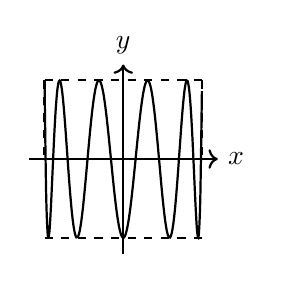
\begin{tikzpicture}
        % 设置绘图参数
        \begin{scope}[thick]
            % 绘制 x 轴和 y 轴
            \draw[->] (-1.2,0) -- (1.2,0) node[right] {$x$};
            \draw[->] (0,-1.2) -- (0,1.2) node[above] {$y$};
            \draw[dashed] (-1,1) -- (1,1);
            \draw[dashed] (-1,-1) -- (1,-1);
            \draw[dashed] (-1,1) -- (-1,0);
            \draw[dashed] (1,1) -- (1,0);
            
            % 绘制切比雪夫多项式 T5(x)
            \draw[domain=-1:1,samples=100,smooth,variable=\x] 
            plot ({\x},{cos(10*acos(\x))});
        \end{scope}
    \end{tikzpicture}
    \caption{最佳逼近的误差等幅振荡}
    \label{fig:besterror}
\end{figure}

当希望在$ [-1,1] $上逼近某多项式$ f $时,如果使用的是某多项式空间$ \mathcal{P}_n $,则如果存在$ g\in \mathcal{P}_n $使得$ f-g $是某一第一类Chebyshev多项式$ T_n(x) $的常数倍,则$ g $是$ f $的最佳逼近,一个简单的例子如下:
\begin{example}
    考虑$ f(x) = ax^3+bx^2+x+c $,下面选取$ a,b,c\in \mathbb{R} $以使得$ \| f \|_\infty $取得最小值。根据上面的分析,我们需要令$ f $是$ T_3 $的常数倍。根据Chebyshev多项式的三项递推关系可知
    \[
        T_3(x) = 2x T_2(x) - T_1(x) = 2x (2xT_1-T_0) - T_1 = 4x^3 -3x,
    \]
    因此要令$ f(x) = -1 / 3 T_3(x) $,所以$ a=-4/3,b=c=0 $。
\end{example}

\end{document}